\documentclass[a4paper,14pt]{article}

\usepackage{comment} % Para comentar várias linhas ao mesmo tempo

%matemática
\usepackage{amsmath}
\usepackage{amssymb}

%diagramação
\usepackage{extsizes}
\everymath{\displaystyle}
\usepackage{geometry}
\usepackage{fancyhdr}
\usepackage{multicol}
\usepackage{graphicx}
\usepackage[brazil]{babel}
\usepackage[shortlabels]{enumitem}
\usepackage{cancel}
\usepackage{textcomp}
\usepackage{tcolorbox}

%tabelas
\usepackage{array} % Para melhor formatação de tabelas
\usepackage{longtable}
\usepackage{booktabs}  % Para linhas horizontais mais bonitas
\usepackage{float}   % Para usar o modificador [H]
\usepackage{caption} % Para usar legendas em tabelas
\usepackage{wrapfig} % Para usar tabelas e figuras flutuantes
\usepackage{xcolor} % Para cores do fundo de tabelas
\usepackage{colortbl} % Para cores do fundo de tabelas

%tikzpicture
\begin{comment}
	\usepackage{tikz}
	\usepackage{scalerel}
	\usepackage{pict2e}
	\usepackage{tkz-euclide}
	\usetikzlibrary{calc}
	\usetikzlibrary{patterns,arrows.meta}
	\usetikzlibrary{shadows}
	\usetikzlibrary{external}
\end{comment}


%pgfplots
\usepackage{pgfplots}
\pgfplotsset{compat=newest}
\usepgfplotslibrary{statistics}
\usepgfplotslibrary{fillbetween}

%colours
\usepackage{xcolor}



\columnsep=2cm
\hoffset=0cm
\textwidth=8cm
\setlength{\columnseprule}{.1pt}
\setlength{\columnsep}{2cm}
\renewcommand{\headrulewidth}{0pt}
\geometry{top=1in, bottom=1in, left=0.7in, right=0.5in}

\pagestyle{fancy}
\fancyhf{}
\fancyfoot[C]{\thepage}

\begin{document}
	
	\noindent\textbf{6FMA116 - Matemática} 
	
	\begin{center}Porcentagem de um número em relação ao outro (Versão estudante)
	\end{center}
	
	\noindent\textbf{Nome:} \underline{\hspace{10cm}}
	\noindent\textbf{Data:} \underline{\hspace{4cm}}
	
	%\section*{Questões de Matemática}
	
	\begin{multicols}{2}
		\noindent Para calcularmos quanto por cento um número $a$ representa de um número $b$, fazemos:
		\begin{center}
		$\frac{a}{b} \cdot 100\%$ \\
		\end{center}
		\noindent\textsubscript{--------------------------------------------------------------------------}
		\begin{enumerate} 
			\item De um total de 40, calcule quanto por cento representa cada número a seguir:
			\begin{enumerate}[a)]
				\item 7 \\\\\\
				\item 1 \\\\\\
				\item 13 \\\\\\
				\item 6 \\\\\\
			\end{enumerate}
			\item Quanto por cento $a$ representa de $b$ quando:
			\begin{enumerate}[a)]
				\item $a = 56$ e $b = 70$? \\\\\\
				\item $a = 3$ e $b = 4$?
				\\\\\\
				\item $a = 7$ e $b = 15$?
				\\\\\\
				\item $a = 7$ e $b = 11$?
				\\\\\\
			\end{enumerate}
			\item Durante um dia, um parque de diversões registrou a visita de 240 pessoas, sendo 150 adultos e o restante crianças. Que porcentagem do total de visitantes desse dia representa o número de crianças? \newpage
			\item \begin{enumerate}[a)]
				\item Flávio tem 3 anos e sua idade representa 37,5\% da idade de seu irmão Rubens. Quantos anos tinha seu irmão quando Flávio nasceu? \\\\\\\\\\\\\\\\\\\\\\\\\\\\\\
				\item A idade de Rubens representa 20\% da idade de seu pai. Quantos anos terá seu pai quando Flávio completar 5 anos? \\\\\\\\\\\\\\\\\\\\\\\\\\\\\\\\
				\item Complete o enunciado com algum número do quadro abaixo e, em seguida, resolva-o com base nos itens anteriores.  \\
				"Bianca, a mãe de Flávio e Rubens, tem \underline{~~~~~~} anos. A idade de Rubens representa qual porcentagem da idade de Bianca?" \\ 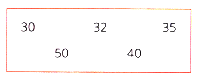
\includegraphics[width=1\linewidth]{6FMA116_imagens/imagem1}
				 \\\\\\\\\\\\\\\\\\\\
			\end{enumerate}
			\textbf{Desafio olímpico} \\\\
			(OBMEP) Em uma festa havia somente 3 mulheres, e 99\% dos convidados eram homens. Quantos homens devem deixar a festa para que a porcentagem de homens passe a ser igual a 98\% do total de participantes?
			\begin{enumerate}[a)]
				\item 3
				\item 30
				\item 100
				\item 150
				\item 297 \newpage
			\end{enumerate}
			% 23 a 28
			\item De um total de 20, calcule quanto por cento representa cada número a seguir:
			\begin{enumerate}[a)]
				\item 1
				\item 3
				\item 9
				\item 13
				\item 19
				\item 21
				\item 25
				\item 70
			\end{enumerate}
			\item Quanto por cento $a$ representa de $b$ quando:
			\begin{enumerate}[a)]
				\item $a = 42$ e $b = 60$?
				\\\\\\
				\item $a = 7$ e $b = 40$?
				\\\\\\
				\item $a = 24$ e $b = 48$?
				\\\\\\
				\item $a = 3$ e $b = 27$?
			\end{enumerate}
			\item Pedro tem 7 anos e Paulo tem 25 anos. Que porcentagem da idade de Paulo representa a idade de Pedro? \\\\\\\\\\
			\item Sabe-se que $x$ representa 38\% de $y$. Quanto vale $\frac{x}{y}$? \\\\\\\\\\\\\\\\\\\\\\\\
			\item Os irmãos Flávio e Guilherme colecionam lápis de cor. Flávio tem 42 lápis e Guilherme tem 35.
			\begin{enumerate}[a)]
				\item Que porcentagem do total de lápis representam os lápis de Flávio? \\\\\\\\\\\\\\\\
				\item Que porcentagem do total de lápis representam os lápis de Guilherme? \newpage
				\item Flávio tem qual porcentagem dos lápis de Guilherme? \\\\\\\\\\\\\\\\\\\\\\\\
				\item Guilherme tem qual porcentagem dos lápis de Flávio? \\\\\\\\\\\\\\\\\\\\\\\\\\\\\\\\\\\\\\\\\\\\\\\\\\
			\end{enumerate}
			\item Durante as férias de verão, Joana decidiu fazer sorvete de frutas com seus filhos. \\
			Para iniciar o processo, eles fizeram a mistura $A$ com 0,2 litro de água e 0,4 litro de suco de abacaxi em uma jarra com capacidade máxima de um litro. \\
			Devido à chegada de alguns amigos, Joana decidiu fazer mais sorvete, acrescentando uma mistura $B$ de água e suco de abacaxi, de forma que a jarra passou a conter um litro. Qual deve ser a porcentagem de água na mistura $B$ para que na mistura final Joana tenha 70\% de suco de abacaxi? \\\\\\\\\\\\\\\\\\\\\\\\
		\end{enumerate}
		$~$ \\ $~$ \\ $~$ \\ $~$ \\ $~$ \\ $~$ \\ $~$ \\ $~$ \\ $~$ \\ $~$ \\ $~$ \\ $~$
	\end{multicols}
\end{document}